\chapter{网络拓扑设计}
%\label{cha:topology}

\section{设计要求}
酒店的外网接ROS的eth0口内网接eth1口,对所有交换机使用hotspot认证,酒店员工办公室的电脑、前
台电脑、特殊用户电脑不需要认证,其他普通用户电脑都需要进行认证。该集成的系统放到酒店一楼的
前台处给客户刷卡取纸条,系统只需要在前台接入酒店内网即可。对酒店普通用户限速$400K$,办公室限
速$600K$,特殊帐号不限速。用户两小时内不上网自动下线。

\subsection{拓扑设备}

\begin{itemize}
\item Raspberry Pi(树莓派),刷卡器,POS打印机三者集成为一个整体,接到一楼网络的前台处。
\item 只需把树莓派接入酒店内网即可工作。
\item 总交换机即为我们的ROS路由,通过该总路由即可管理整个酒店网络
\item 比如一楼的用户要上网,通过刷卡然后取走纸条即可上网
\item 树莓派实时控制ROS路由
\end{itemize}

\subsection{拓扑结构}

这里显示了一楼前台处的树莓派+刷卡器+打印机三者为一个整体,连接外网的是ROS,ROS的eth1接入酒
店内网交换机。

其他终端用户上网都需要经过ROS的认证,通过到前台刷卡然后如果是入住酒店打印机打印出一张纸条,
客户取走纸条后接入酒店网络弹出认证界面,按照纸条上的用户名密码输入上网。

客户退房的时候在刷一次卡,这次打印机不会出纸条,听到嘀的一声后就注销了,纸条上的用户名和密
码作废。

通过在ROUTER OS中设置IP$\rightarrow$Hotspot$\rightarrow$Ip Bindings设置不需要认证的ip,但是
对于要批量设置的话可以使用其中一个不需要认证的ip接入办公室的路由器,办公室就不用经过认证了,
办公室限速$600K$只需要限制这一个ip的网速就可以了。对于普通用户的限速在Queues里面写规则限制。

在Queues里面写限速规则
\begin{enumerate}
\item ROS单IP限速
  \begin{enumerate}
  \item 首先登陆WINBOX,点击QUEUES,这个就是限速窗口,现在是空白的,再点击“红色+号”新建一个
    限速规则。
  \item 名字自己起,最好是一看就明白的,target upload:目标上传;target download:目标下载。
    这里要说明一下,在ROS里表达的流量值单位是位(bit),而我们平时说的申请了$2M$的ADSL,这
    个$2M$,单位也是位(bit),但是我们说的下载速度多少$K$,指的单位是字节,它们之间的比例
    是:8位(bit)$=$1字节,所以,上传$128k/8=15K$(请注意大小写:$k*8=K$)。下面还可以设置
    每个星期几限速,全打上就是每一天都限的意思。
  \item 当我们设置完了限制的速度后,我们还要设置要限制的电脑IP,才能实现效果哦。点
    击advanced(高级)栏,在dst. address处输入你要限制速度的IP地址,然后点OK完成。
  \item ROS限速的确很好用,限了多少就是多少,非常准确的。
  \end{enumerate}
\item ROS网段限速
  \begin{enumerate}
  \item 首先登陆WINBOX,点击:system-scripts
  \item 通过脚本来对整个网段限速,先点“红色+号”,新建一个脚本,名字你喜欢,在SOURCE处粘贴源代码   
    \begin{minted}[fontsize=\small,
      linenos=true,numbersep=2pt,
      frame=leftline,framesep=3pt,rulecolor=\color{lightgray},
      xleftmargin=10pt
      ]{bash}
      :for myip from 2 to 250
      do={
        /queue simple add name=(“限192.168.1.” . $myip . “”)
        target-address=(“192.168.1.” . $myip . “/32″)
        limit-at=0/0 max-limit=150000/1024000
      }
    \end{minted}
  \item 即可以192.168.1.2-250限速
  \item 创建了脚本,还要运行才能生效。选中要运行的脚本,再点击RUN…,这样整个网段都可以实现
    统一限速了。
  \end{enumerate}
\end{enumerate}

酒店网络拓扑如图~\ref{fig:hotel}所示。注意,这里仅说明了酒店的一楼网络,其他楼层同样需要经
过认证才可以上网,树莓派接入酒店内网任意位置都可以进行啥卡认证,客户的笔记本的电脑、PC、智
能手机都需要认证上网,办公室的位置没有标出。

\begin{figure}
  \centering
  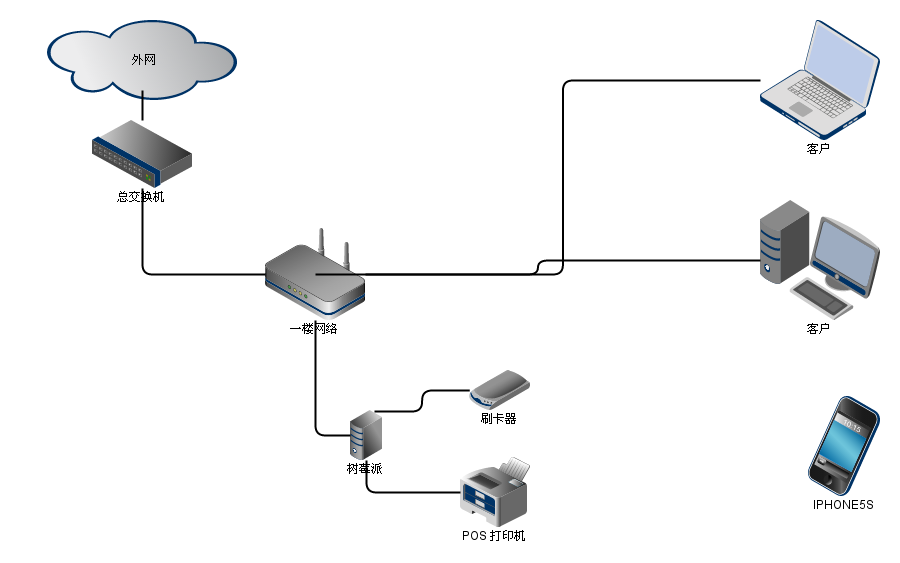
\includegraphics[width=.9\textwidth]{pic/hotel.png}
  \caption{酒店拓扑}
  \label{fig:hotel}
\end{figure}

%%% Local Variables: 
%%% mode: latex
%%% TeX-master: "../thesis"
%%% End: 
